\documentclass[twocolumn,desyfonts,twoside]{desypaper}  %% do not change these
%\usepackage{a4wide,makeidx,english,babel}
\usepackage{a4wide,makeidx}
\usepackage[english]{babel}
\usepackage{amsmath,amsfonts,verbatim,graphicx,float}

\usepackage{color}
\usepackage{alltt}
\usepackage[latin1]{inputenc}


\usepackage{fancyhdr, moreverb}


\def\CJT{CheckboxTree}


\newcommand{\desc}[1]{\item[\textbf{#1}]}
\newcommand{\ttt}[1]{\texttt{#1}}

\newcommand{\bc}{\begin{center}}
\newcommand{\ec}{\end{center}}
\newcommand{\be}{\begin{equation}}
\newcommand{\ee}{\end{equation}}
\newcommand{\bea}{\begin{eqnarray}}
\newcommand{\eea}{\end{eqnarray}}
\newcommand{\bi}{\begin{itemize}}
\newcommand{\ei}{\end{itemize}}
\newcommand{\bd}[1]{\begin{dinglist}{#1}}
\newcommand{\ed}{\end{dinglist}}
\newcommand{\bt}{\begin{tabular}}
\newcommand{\et}{\end{tabular}}



\begin{document}

\author{L.~Bigagli, E.~Boldrini}
\title{\CJT{}}

\address{IMAA-CNR \\ bigagli@imaa.cnr.it, boldrini@imaa.cnr.it}

\abstract{ We describe the \CJT{}, a Swing-based tree with a
checkbox in each of its nodes, similar to those commonly found in
installers (and unfortunately missing in Swing). We wrote the
component building upon Swing design, and spiced it up with features
like configurable styles of check propagation and greyed checkboxes
when a subtree is not completely (un)checked. We give insights about
the component design, along with usage examples, documentation and
source code.}

\maketitle


\section{Introduction}

\begin{figure*}[]
\bc
\includegraphics[angle=0,width=0.4\textwidth]{CheckboxTree.png}
\caption{The \CJT{} in action. Checked, selected and greyed paths
are visible.} \label{fig.demoApp} \ec
\end{figure*}


The \CJT{} component is a Swing-based tree with a checkbox in each
of its nodes, more precisely a JTree with a JCheckbox in each of its
node (see figure \ref{fig.demoApp}). Similar components are commonly
found in installation GUIs, preferences windows, etc. Unfortunately
Java Swing does not include such a component. We instead knew about
other free Swing-based implementations, (e.g. \cite{santosh},
\cite{sample}) but they lacked the features and the flexibility that
we needed, and that we have added to this new GPL-licensed
component. Moreover we wrote the code trying to keep a
\emph{Swing-compatible} approach and trying to write a robust and
customizable component.

In the next sections we describe the \CJT{} and relate it to the
relevant Swing components, particularly to the JTree-related
classes. Details about the architecture and implementation are also
given. Finally we describe some known limitations and some ideas for
possible improvements.

\section{Swing JTree}
In this section we try to describe the behavior of the \CJT{}. In
doing this we recall the Swing JTree language and concepts that will
help us for the description, we'll also introduce concepts like the
greyness and the checking of a tree that are not present in the
standard JTree implementation.

\subsection{JTree terms}
As described in the Swing documentation \cite{swing-jtree} a
\emph{JTree} is a control that displays a set of hierarchical data
as an outline.

A specific node in a tree can be identified either by a TreePath or
by its display row.

A \emph{TreePath} is an object that encapsulates a node and all of
its ancestors.

A JTree has a TreeModel for managing its data model, following the
well-known model-view-controller pattern.

\subsection{Using the \CJT{}}

A \CJT{} user has to write his/her tree extending the \CJT{} class
and (in case the provided DefaultCheckboxTreeCellRenderer is not
sufficient) implement the CheckboxTreeCellRenderer with a custom
renderer.

A key feature of our component is that the user can continue to work
with his/her defined node objects, which don't need to implement a
common interface like in other solutions (e.g. a CheckableTreeNode
interface). This can speed up the integration of the component in
the existing code.

\section{\CJT{}}

\subsection{The Checking}
In the \CJT{} all the tree nodes have a checkbox that can be checked
by the user by clicking on it if is enabled. A checked node is
plainly a tree node that has a check on its checkbox and a checked
TreePath is a TreePath that have its last component checked. For
\emph{checking} we mean the set of all the TreePaths of a JTree that
are checked.


\subsection{The Greyness}
In our component when a checkbox has a grey background it means that
exists at least one of its descendants with a checking status
different from itself (e.g. a checked directory that has at least
one file unchecked is grey rendered).

When the checked property of a checkbox changes we must maintain the
consistency of this property (un)greying the checkboxes that are
influenced by the changing (possibly some ancestors or the
children).

\subsection{Checking mode}
A relevant feature implemented in our component is the possibility
of changing the propagation style of the checking (and possibly
writing new ones). For checking mode we mean the way the check is
propagated to the other checkboxes after a user has clicked on one
of them. We have implemented four different styles of propagation
that we are going to describe. They propagate the checking in
different modes and in doing so they also change the greying
property of influenced checkboxes if needed with checking
mode-optimized procedures.
\begin{itemize}

\item
The \emph{simple checking mode} toggles the checking of the just
clicked checkbox only.

\item
The \emph{down recursive checking mode} toggles the checking of the
just clicked checkbox and propagates it to other checkboxes in a
down recursive style. This means that if the clicked checkbox is now
checked all the descendants will be checked, in the other case all
the descendants will be unchecked.

\item
The \emph{full recursive checking mode} propagates the checking not
only to descendants but also to ancestors of the clicked TreePath.

In the first part this mode behaves exactly like the down recursive
mode.

In a second \emph{up recursive} part it also propagates the checking
to ancestors. In particular if the clicked checkbox is now unchecked
all the ancestors will be unchecked. If the clicked checkbox is
instead now checked we control the first ancestor: if it has all
children checked we checks it and so on with all the ancestors.

\item
The \emph{checked full recursive checking mode} behave similar to
the full recursive checking mode.

In the first part this mode behaves exactly like the down recursive
mode.

In a second \emph{up recursive} part it propagates the checking to
ancestors. In particular if the clicked checkbox is now checked all
the ancestors will be checked. If the clicked checkbox is instead
now unchecked we control the first ancestor: if it has all children
unchecked we uncheck it and so on with all the ancestors.

\end{itemize}



\section{Implementation insights}


\begin{figure*}[]
\bc
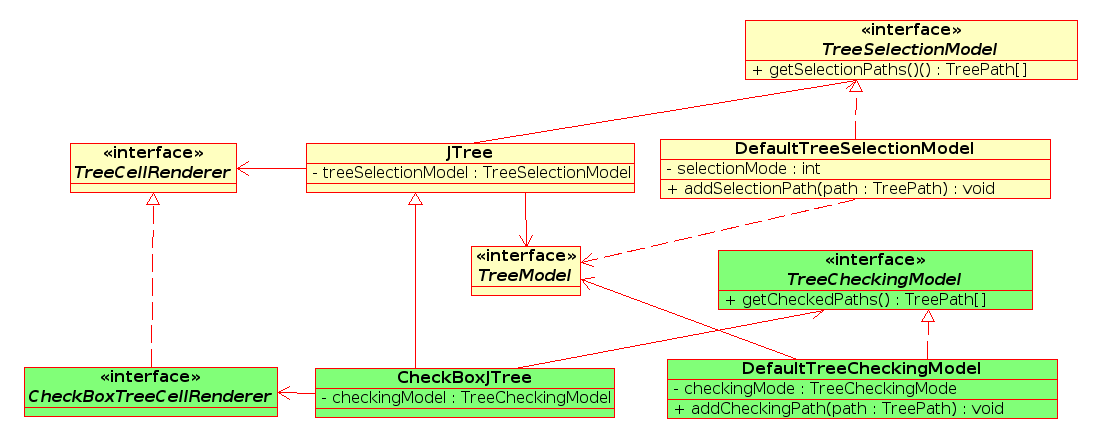
\includegraphics[angle=0,width=1\textwidth]{dia-small-right.png}
\caption{The similarity between pre-existent Swing architecture
(yellow classes) and our new one (green classes).}
\label{fig.classDiagram} \ec
\end{figure*}


\subsection{Swing similarity}
The main new property added to the initial JTree is the management
of the checking. For this scope we wrote the TreeCheckingModel
class. We provided this class with an API similar to the Swing
TreeSelectionModel, that is the class that in Swing manages the
selection. This gives the final user easiness of use, assuming that
is already familiar with Swing. The similarity is extended to the
classes hierarchy and relations structure as it's possible to see in
the UML diagram in figure \ref{fig.classDiagram}.


The similarity between the Swing classes that manage the selection
(in yellow) and the new classes for the checking management (in
green) is highlighted with two dotted red lines.

We can also see that a JTree uses a TreeModel, a TreeCellRenderer
and a TreeSelectionModel. The \CJT{} extends the JTree adding to it
the capability to use a TreeCheckingModel. Moreover a \CJT{} needs
an implementation of CheckboxTreeCellRenderer, that is a
TreeCellRenderer that display a checkbox or similar components
inside each tree node (we provide a DefaultCheckboxTreeCellRenderer
with a JCheckbox). In general children classes has to implement the
method \texttt{boolean isOnCheckbox(int x, int y)} that given the
coordinates of a user click returns if the click was on the
checkbox. In that case the JTree (listener of the user clicks) will
modify the checking using the TreeCheckingModel.


\subsection{CheckboxTreeCellRenderer}


\begin{figure*}[]
\bc
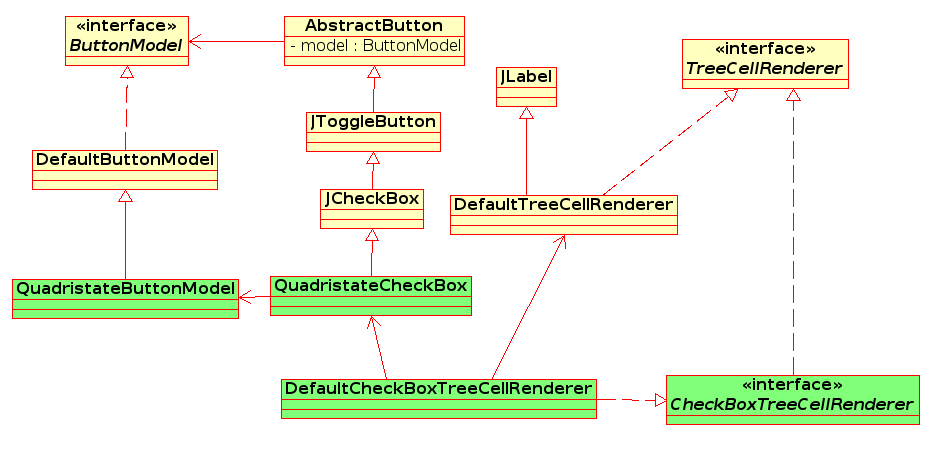
\includegraphics[angle=0,width=1\textwidth]{dia-small-left.png}
\caption{Classes diagram of the QuadristateCheckbox neighborhood.}
\label{fig.quadristate} \ec
\end{figure*}

We needed a TreeCellRenderer capable of displaying a checkbox in
four states: checked, unchecked, grey checked and grey unchecked.
Thus we have implemented a QuadristateCheckbox that supports Look
and Feel and displays the four states managed now by a new model
called QuadristateButtonModel, see figure \ref{fig.quadristate} for
the classes hierarchy. In point of fact we have used an hack
implementing a quadristate checkbox for displaying the two new
states with a normal JCheckbox.



%\onecolumn


%\twocolumn


\section{Considerations and future work}
Some limitations of this component are known and we plan to fix them
in future releases.

\begin{itemize}
\item
The main limitation regards the component performance when dealing
with very full trees. For example if the checking propagation mode
is set on down recursive and we perform a click on a node with many
descendants the GUI freezes for the time needed to insert all the
sub paths that become checked in the relevant sets. The information
that all the descendants of a node are checked could instead be
memorized putting only the ancestor in an appropriate set and thus
cutting down the time of execution.
\item
The rendering of the grey checked state in the checkboxes is given
by setting both the armed and pressed property to true in the model,
the price is that we can't use rollover events on the new
checkboxes. A better implementation of QuadristateCheckbox would
maintain the capability of managing rollover events and display them
in an appropriate way.
\end{itemize}

\bibliographystyle{plain}
\bibliography{CheckboxTree}

\end{document}
